\documentclass[a4paper,10pt]{article}
\usepackage[margin=1.25in]{geometry}
\usepackage[utf8]{inputenc}
\usepackage{graphicx}

\usepackage[dvipsnames]{xcolor}
\usepackage{fancyvrb}

% redefine \VerbatimInput
\RecustomVerbatimCommand{\VerbatimInput}{VerbatimInput}%
{%fontsize=\footnotesize,
 %
 frame=lines,  % top and bottom rule only
 framesep=2em, % separation between frame and text
 rulecolor=\color{Gray},
 %
% label=\fbox{\color{Black}data.txt},
 labelposition=topline,
 %
 %commandchars=\|\(\), % escape character and argument delimiters for
                      % commands within the verbatim
 %commentchar=*        % comment character
}



%opening
\title{Introduction to ABC-SMC}
\author{Thomas J. Hladish}

\begin{document}

\maketitle

\begin{abstract}
Mathematical models are a valuable tool in many fields for understanding system dynamics, making predictions, and evaluating potential intervention strategies.  Models need to be fit to and validated against observed data, however, in order to say whether a model is good.  Model fitting, or estimating parameter values, can be technically challenging for all but the simplest models because of the computational and statistical complexity of the procedure.  This guide introduces the concept of Bayesian parameter estimation, and provides a basic tutorial for AbcSmc, a C++ toolkit that samples parameter space, compares output from a user-provided model to observed metrics using partial least squares, and calculates convergence statistics.  Although AbcSmc can be used in a distributed computing environment, the focus here is on personal computer applications for simulations not implemented in C++.


\end{abstract}

\section{A game of chance}
Consider a simple game:  I have some number of standard, six-sided dice.  I roll them, add up the values on their top faces, and get 7.  How many dice do I have?

Of course, you can't know for sure; I could have two dice, and rolled a 3 and a 4, or maybe I have five and I rolled 1, 1, 1, 1, and 3.  What you can say is the most \textit{likely} number of dice I have, given assumptions about how my dice work, and you can further calculate the likelihood of the possible alternatives.

Let's first define a model of the process.
\begin{enumerate}
 \item Write down some mathematical statements that describe the process of summing the faces of some number of rolled dice.
 \item Write an R function that takes a number of dice as an argument, ``rolls'' that number of dice, and returns the sum.
\end{enumerate}

Note that you have likely made some assumptions.  For example, you probably made the\textemdash very reasonable\textemdash assumptions that my dice did not somehow end up stacked or balanced on edge, so that I counted either fewer or more faces than the number of dice I rolled.  While these things are in principle possible, they are unlikely and presumably improbable outcomes.  Even for a game as simple as this, the model isn't reality, and assumptions make the difference.

In order to answer the question of how many dice I rolled in this instance, we need to characterize the realm of possibilities.

\begin{enumerate}
 \item What is the minimum number of dice I have?
 \item What is the maximum number of dice I have?
 \item Are all numbers of dice equally likely? (Without more information from me, you need to assume that they are.)
\end{enumerate}

In this model, there is only one thing to vary, only one \textit{parameter}: the number of dice. The questions above characterize the \textit{prior probability distribution}, often just \textit{prior}, for that parameter.  Sometimes choosing a prior is difficult or seems arbitary, but it is an important part of articulating the assumptions of your model.  Note in this case, the range of the prior is constrained by having observed a sum of 7, but the shape of the prior, that all possible quantities of dice are equally likely, is less justified.

For each of the possible number of dice, run the dice summing function you wrote 10,000 times.  What fraction of the 10,000 times do you get a sum of 7?

% faceSum <- function(ndice){
%   sum(sample(6,ndice,replace=T))
% }
% 
% p <- sapply(2:7, function(d,nrolls=10^6,target=7){
%   rolls <- replicate(nrolls,faceSum(d))
%   sum(rolls==target)/nrolls
% })
% 
% # p = c(0.166329, 0.069855, 0.015400, 0.001944, 0.000133, 0.000003)

\begin{figure}[h]
 \centering
 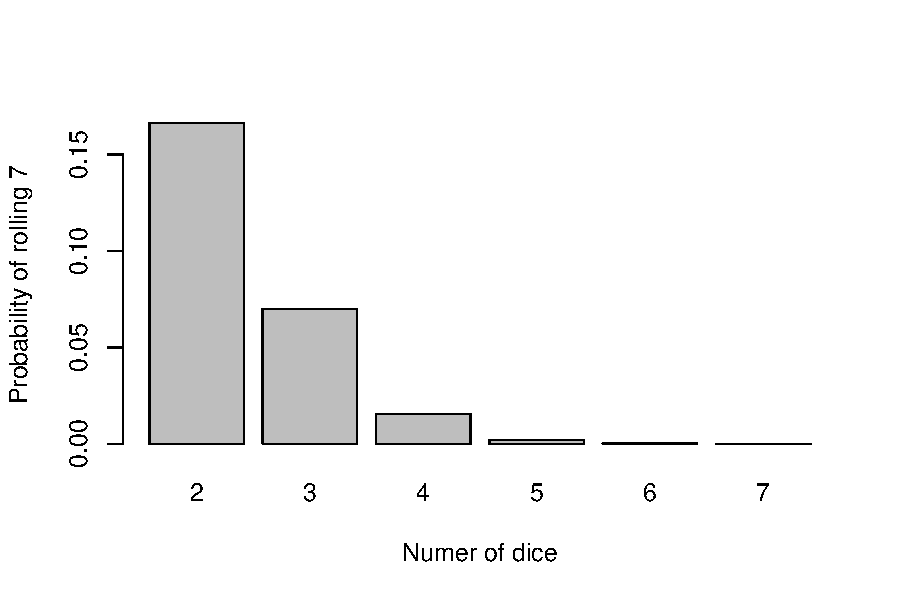
\includegraphics[width=0.80\textwidth]{./simple_roll.pdf}
 % simple_roll.png: 1200x800 pixel, 160dpi, 19.05x12.70 cm, bb=0 0 540 360
 \caption{The approximate likelihood of each possible number of dice, given that they must sum to 7.  In a Bayesian context this would be called the (unnormalized) posterior probability distribution.}
 \label{fig:dice_likelihood}
\end{figure}

Plotted as a bar chart, you should get results that look similar to Figure 1.  This is the \textit{posterior probability distribution}, or \textit{posterior}.  The prior describes your expectations or knowledge about a parameter before accounting for some piece of information, in this case how many dice you expect me to have before you account for them summing to 7, and the posterior describes how many dice you think I have after taking their sum into account.  From the posterior, we can see that the most likely number of dice is 2, with a mean that is somewhat higher, around 2.4.  Note that the probabilities in Figure 1 are not normalized, meaning they do not sum to one.

This dice exercise can be solved analytically, so we didn't need to use a computational approach, but there are many models where analytical solutions are difficult or impossible.  For those models, we use an approach called approximate Bayesian computation, or ABC.  The dice exercise we just did is ABC applied to a simple problem.  Let's consider a version of the problem that is more complicated.

\section{Increasing complexity}
In the last game, we assumed that the dice were standard, six-sided dice.  What if we allow the dice to have an arbitary number of sides?  This presents an inference problem, because a change in the sum I report to you could be due to a change in the number of dice or a change in the number of faces they have.

\begin{figure}[h]
 \centering
 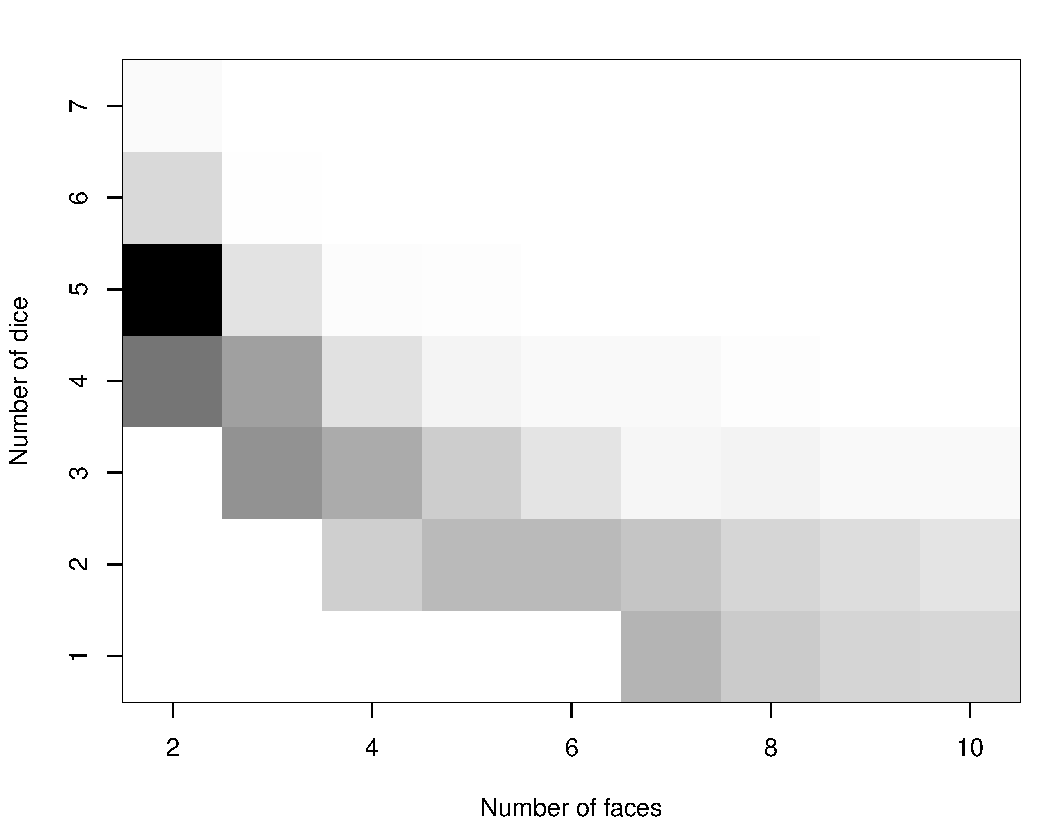
\includegraphics[width=0.80\textwidth]{./dice_vs_faces.pdf}
 \caption{The 2-dimensional approximate posterior probability of each number of dice and each number of sides in the prior, given that they must sum to 7.}
 \label{fig:dice_likelihood}
\end{figure}


\pagebreak
\appendix
\section*{Appendices}
%\addcontentsline{toc}{section}{Appendices}
\renewcommand{\thesubsection}{\Alph{subsection}}

\subsection{Configuration file template}
TODO - Decide which features to describe and indicate required/optional fields
\begin{Verbatim}[commandchars=\\\{\}]
\{
    "smc_iterations"            : 8,
    "num_samples"               : 1000,
    "predictive_prior_fraction" : 0.1,
    "pls_training_fraction"     : 0.5,

    "database_filename"         : "dice.sqlite",

    "parameters" : [
        \{"name"       : "parameter 1",
         \textit{"short_name" : "par1",}
         "dist_type"  : "UNIFORM",
         "num_type"   : "INT",
         "par1"       : 1,
         "par2"       : 1000\},

        \{"name"       : "number of sides",
         \textit{"short_name" : "nsides",}
         "dist_type"  : "UNIFORM",
         "num_type"   : "INT",
         "par1"       : 1,
         "par2"       : 1000\}
    ],

    "metrics" : [
        \{"name"       : "dice_sum",
         "num_type"   : "INT",
         "value"      : 314\},

        \{"name"       : "standard deviation",
         \textit{"short_name" : "dice_stdev",}
         "num_type"   : "FLOAT",
         "value"      : 3.45844\}
    ]
\}
\end{Verbatim}

\pagebreak

\subsection{Example configuration file}
\VerbatimInput{dice_config.json}
\pagebreak

\subsection{Example R simulation}
\VerbatimInput{dice_abc.R}
\pagebreak

\end{document}
